\chapter{\label{ch:MeasurementCorrections}Measurement Corrections}

\chapauthor{Darrel J. Conway}{Thinking Systems, Inc.}

To be written.

\section{Introduction}

\section{Additive Corrections}

\section{Event Based Corrections}

\begin{figure}
\begin{center}
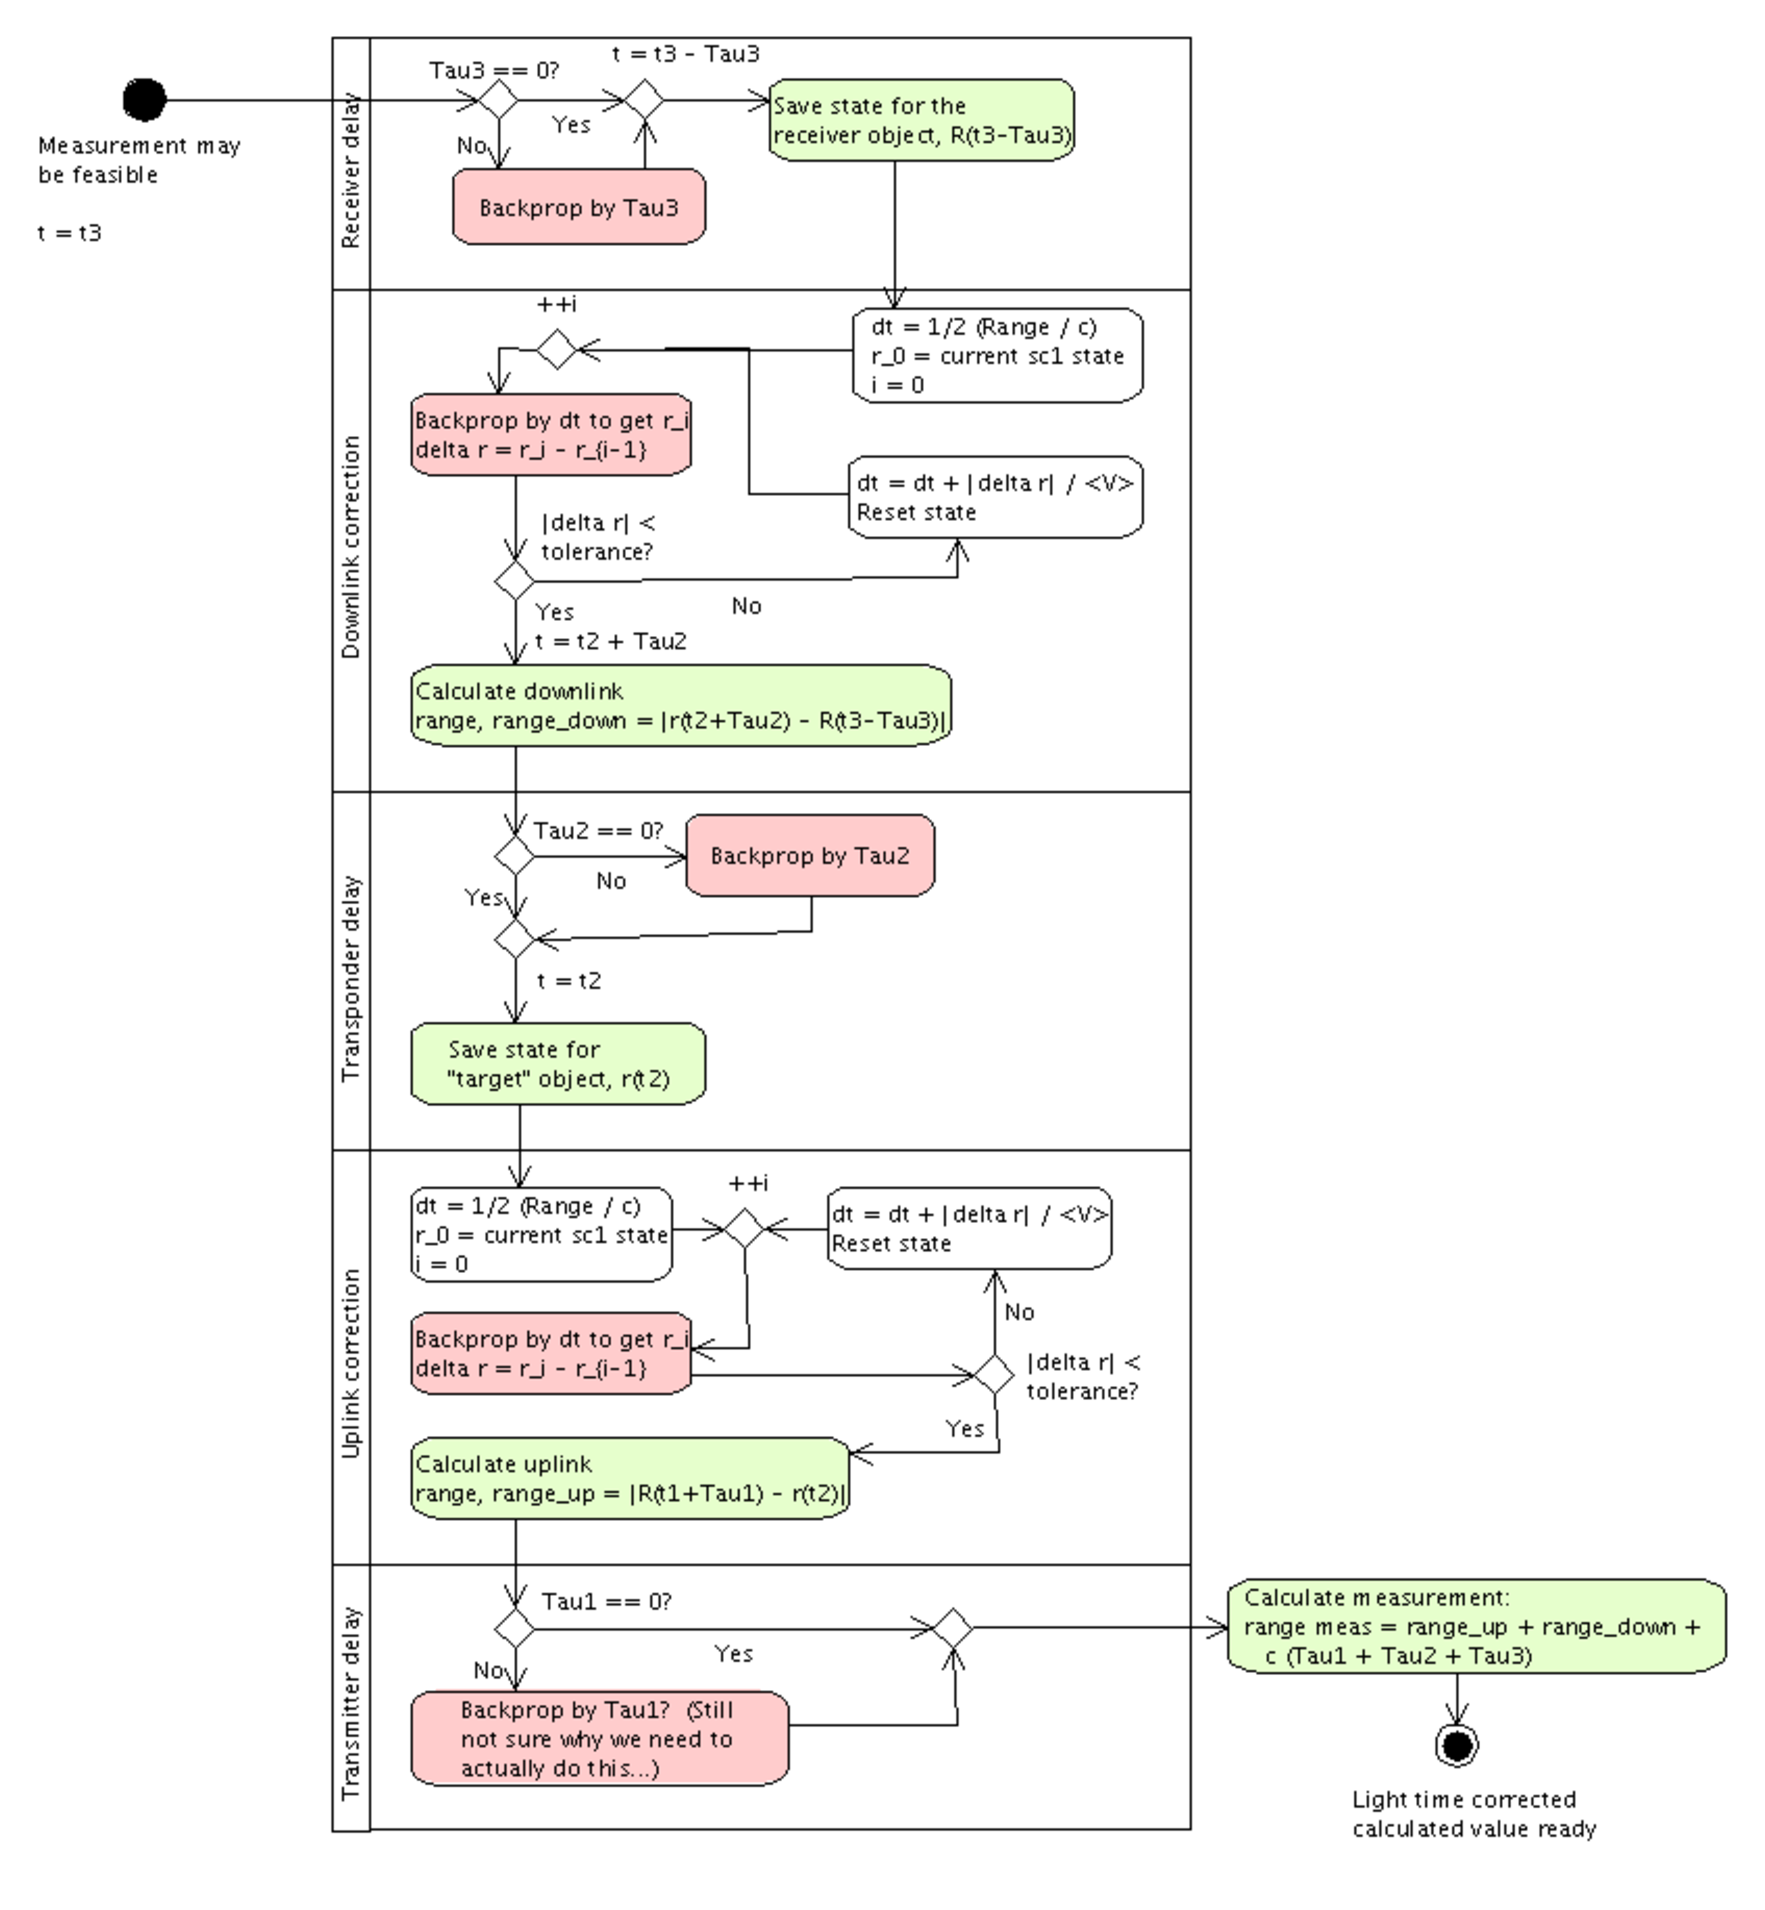
\includegraphics[scale=0.52]{Images/EventLocationLightTimeCorrection.eps}
% EventLocationLightTimeCorrection.png: 831x901 pixel, 72dpi, 29.32x31.79 cm, bb=0 0 831 901
\caption{Steps in Light Time Correction: Two Way Range}
\end{center}
\end{figure}


\begin{figure}
\begin{center}
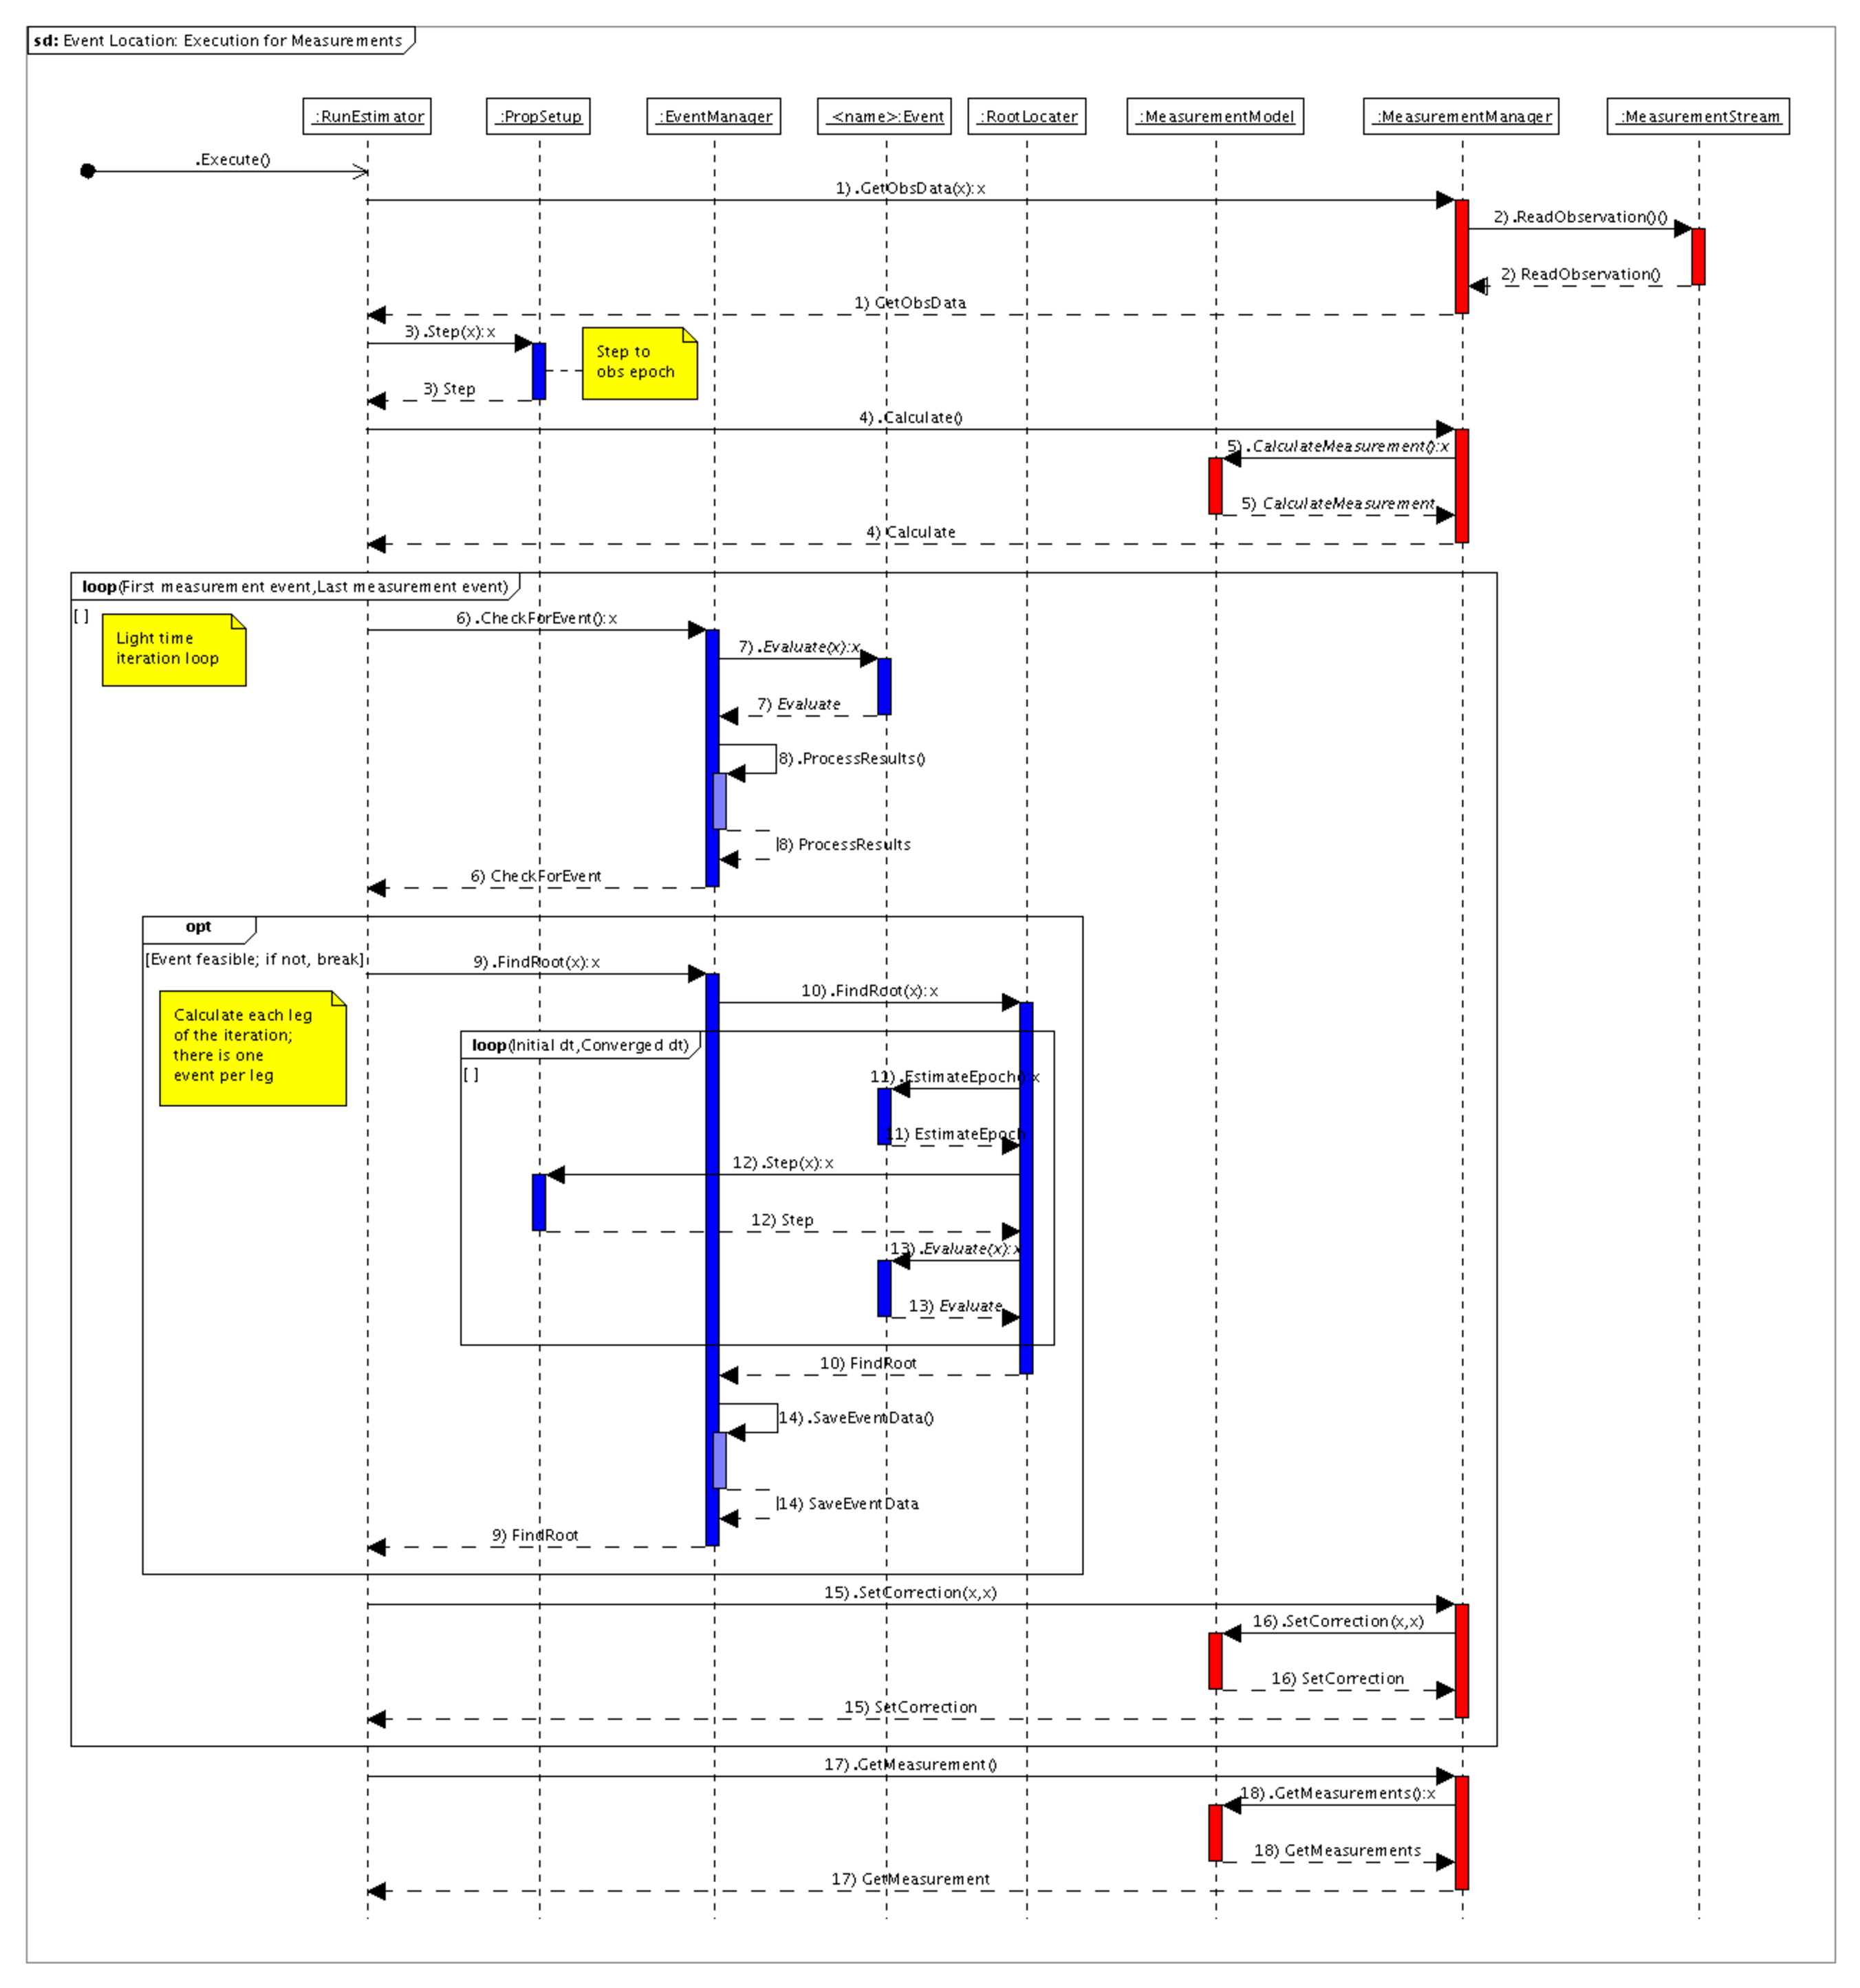
\includegraphics[scale=0.36]{Images/EventLocationExecutionforMeasurements.eps}
% EventLocationExecutionforM...ts.png: 1282x1371 pixel, 72dpi, 45.23x48.37 cm, bb=0 0 1282 1371
\caption{\label{fig:MeasurementLocationSD}Event Location for Measurements}
\end{center}
\end{figure}